%% -*- latex -*-

%%----------------------------------------------------------------------
\title{
\includegraphics[height=2.5cm]{files/ansible-logo-2.png}\\[1ex]
%	\hspace{0.5cm}\textbf{Ansible}\\[1ex]
       \normalsize{Configuration Management \&{} IT-Automation}}
\author[Andreas Härpfer]{Andreas Härpfer \\
  {\scriptsize \href{mailto:andreas.haerpfer@consol.de}
  	            {\nolinkurl{(andreas.haerpfer@consol.de)}}}}
\institute{Consol-Akademie}
\date{2014-05-27}

%% PDF properties
\subject{Ansible -- Configuration Management \&{} IT-Automation}
%\keywords{}

\begin{document}

% Load default settings for lstlisting environment.
%% Default style for the lstlisting environment.
\lstset{ %
  language=Clean,				% language
  basicstyle=\scriptsize\ttfamily,		% fontsize and style
  xleftmargin=0pt,				% listing indentation
  %xleftmargin=1.5em,				% listing indentation
  %numbers=left,
  numberstyle=\tiny,
  %stepnumber=1,				% lineno stepping
  %numbersep=5pt,                  		% sep of lineno-s
  backgroundcolor=\color{LightGray},  		% requires \usepackage{color}
  showspaces=false,
  showtabs=false,
  %% Draw a box around the listing and change BG color.
  %frame=single,				% draw frame
  frame=lrtb,
  framesep=4pt,
  %framerule=1pt,
  tabsize=8,
  captionpos=b,
  breaklines=true,				% auto linebreaking
  breakatwhitespace=true,			% break only at whitespace
}



%%----------------------------------------------------------------------
\begin{frame}[plain]
  \titlepage
\end{frame}

\begin{frame}[plain]
  \begin{quote}
  {\Large ``I can't explain philotic physics to you. Half of it nobody
  understands anyway. What matters is we built the ansible.''\par}

  \vspace{2ex}
  \hfill -- Ender's Game
  \end{quote}
\end{frame}

\begin{frame}{Agenda}
  \tableofcontents
\end{frame}

%%----------------------------------------------------------------------
\section{Configuration Management, IT-Automation und Ansible}

\begin{frame}{Configuration Management: Generationen}
  \begin{table}
%    \small
    \setlength{\aboverulesep}{0pt}
    \setlength{\belowrulesep}{0pt}
    \setlength{\extrarowheight}{0.8ex}
    \begin{tabularx}{\textwidth}{|X|XX|XX|}
      \toprule
      \rowcolor{Gray}%
      \mc{1}{|c|}{\textbf{1st Gen.}} &
      \mc{2}{c|}{\textbf{2nd Gen.}} &
      \mc{2}{c|}{\textbf{3rd Gen.}}%
      \bstem\\

      \midrule
      \rowcolor{LightBlue}%
      \emph{cfengine} & \emph{Puppet} & \emph{Chef} &
      \emph{Salt} & \emph{Ansible} \\

      \midrule
      1993 	& 2005 		& 2009 		& 2011	& 2012 \\
      C 	& \mc{2}{c|}{Ruby}		& \mc{2}{c|}{Python} \\
      eigene~DSL& \mc{2}{c|}{Ruby(ish) DSLs} 	& \mc{2}{c|}{YAML} \\
      
      Agent	& Agent		& Agent		& Agent%
      \footnote{Agent-less möglich aber noch "`not for production"'
      (2014-05).} & \tblue{SSH-only} \\
      
      Pull	& Pull		& Pull		& \tblue{Push} &
      \tblue{Push}\footnote{Mit \emph{ansible-pull} ist mittlerweile auch ein
      Pull-Verfahren möglich.}%
      \bstem\\
      \bottomrule
    \end{tabularx}
  \end{table}
\end{frame}


\begin{frame}{Configuration Management: Push vs.~Pull}
  \begin{block}{Pull}
    \begin{itemize}
      \item Dynamisches Environment.  Neue Systeme holen sich ihre
      Konfig (periodisch) selbst \dots{}\\ Aber wie kommt der Agent auf
      das System?

      \item Skalierbarkeit \dots{} aber keine Kontrolle über Lastspitzen.

      \item Asynchrones Fehlerverhalten, Fehler sind verteilt.
    \end{itemize}
  \end{block}

  \pause
  \begin{block}{Push}
    \begin{itemize}
      \item Einfaches Bootstrapping: bare server setup \dots{}\\ Aber
      wie erkennt man neue Systeme?

      \item Pushes können fehlschlagen.

      \item Synchrones Fehlerverhalten, Fehler lokal auf dem Master.

      \item Einfacheres Development: Änderungen einfach ausprobieren,
      keine Verbindungen von außen, \dots
    \end{itemize}
  \end{block}

%  \pause
%  Der Trend geht zu "`Push"' \dots
\end{frame}


\begin{frame}{Was ist Ansible?}

  Ansible ist \dots\footnote{``An ansible is a fictional machine capable
  of instantaneous or superluminal communication. [\dots] It can send
  and receive messages to and from a corresponding device over any
  distance whatsoever with no delay.''
  (\href{https://en.wikipedia.org/wiki/Ansible}{Wikipedia})}

  \pause
  \begin{itemize}
    \item Ein \emph{3rd generation configuration management \&{} IT
    automation tool}.

    \item Geschrieben in Python.

    \item Agenten-los, Kommunikation rein über SSH.

    \item Top-5 Github-Projekt in 2013, aktuell immer noch Top-10
    Python-Projekt.

    \item Aktuelle Version 1.6, released Mai 2014.

    \item $> 230$~Module out of the box.
  \end{itemize}
\end{frame}


\begin{frame}{\dots{} mehr als nur Config Management!}
  \begin{block}{"`Command Blaster"'}
    \begin{itemize}
      \item Ein Kommando auf eine ganze Gruppe von Hosts loslassen.
      \item Quick and dirty, à la parallele SSH.
    \end{itemize}
  \end{block}
  
  \begin{block}{Orchestration\footnotemark}
    \begin{itemize}
      \item Workflow-Beschreibungen.
      \item Andere Tools triggern, Ausführungsreihenfolge festlegen.
      \item Komplexe Multi-Tier Deployments, Rolling Updates, \dots
    \end{itemize}
  \end{block}

  \begin{block}{Klassisches Configuration Management}
    \begin{itemize}
      \item Zustandsbeschreibung
      \item Konvergenz, Idempotenz
    \end{itemize}
  \end{block}

  \emph{Fun Fact: Es gibt Firmen, die Puppet mit Ansible orchestrieren.}
  \footnotetext{\url{http://www.ansible.com/blog/orchestration-you-keep-using-that-word}}

\end{frame}


%% Die Google-Statistik ist nicht wirklich zuverlässig, da es ein
%% Kommunikationsprojekt namens Ansible von Siemens gibt, das hier
%% leider mit rein spielt.

%\begin{frame}{Google-Trends: Ansible vs SaltStack}
%  \includegraphics[width=\textwidth]{files/google-trends.png}
%
%  rot = Ansible
%
%  blau = SaltStack
%\end{frame}


%%----------------------------------------------------------------------
\section{Ansible: Getting Started}

\begin{frame}{Requirements}

  \begin{block}{Control Machine}
    \begin{itemize}
      \item Unix\emph{oides} OS (kein Windows)
      \item Python $\ge$~2.6
    \end{itemize}
  \end{block}

  \begin{block}{Managed Nodes}
    \begin{itemize}
      \item SSH
      \item Python $\ge$~2.4
      \item ggf.~\emph{python-simplejson} (falls Python $<$~2.5)
    \end{itemize}
  \end{block}
\end{frame}


\begin{frame}[fragile]{Installation}
  \begin{itemize}
    \item Python Virtualenv (bevorzugte Methode):

    \begin{lstlisting}
$ virtualenv ansible-venv
$ source ./ansible-venv/bin/activate
(ansible-venv) $ pip install ansible
Downloading/unpacking ansible
  Downloading ansible-1.6.2.tar.gz (649kB): 649kB downloaded
  Running setup.py egg_info for package ansible

  [...]

 Successfully installed ansible paramiko jinja2 PyYAML pycrypto ecdsa markupsafe
Cleaning up...
    \end{lstlisting}

    \item Package Manager des OS (aktuelle Version?).

    \item Direkt per Github-Clone.
  \end{itemize}
\end{frame}


\begin{frame}[fragile]{Das Inventory}
  \lstinputlisting[basicstyle=\tiny\ttfamily]{demo/hosts}
  \blfootnote{Dynamische Inventories kommen später.}
\end{frame}


\begin{frame}[fragile]{Ad-hoc Command Mode}
  Kommandos mittels Ansible auf mehreren Hosts ausführen:
  \begin{itemize}
    \item Gruppen und Patterns möglich.
    \item Direkter Aufruf von Modulen möglich.
    \item Auth-Parameter, Sudo, Output-Logging, Parallelisierung, \dots
  \end{itemize}
  \vspace{1ex}
  \begin{lstlisting}
$ ansible -i hosts all -m ping
$ ansible -i hosts all -a id -f10
$ ansible -i hosts *01* -a uptime -o

$ ansible dmz -a 'ntpq -p' --limit web*
$ ansible appsrv01 -m copy \
  -a 'src=./hosts dest=/tmp/testfile mode=600 owner=admin'
$ ansible web -u root -m shell \
  -a 'ps auxw | grep apache | grep -v grep'
  \end{lstlisting}
  
\end{frame}


%%----------------------------------------------------------------------
\section{Ansible: Module, Rollen und Playbooks}

\begin{frame}{Module}
  \begin{itemize}
    \item Parametrisierte Bausteine für komplexere Aktionen.
    \item Können in beliebiger Sprache selbst geschrieben werden.
    \item Schnittstelle via JSON-Datenstruktur.
    \item $> 230$ Module für die gängigsten Anforderungen bereits
    enthalten:\footnote{\url{http://docs.ansible.com/modules_by_category.html}
    }\\[1ex]

    Package Management, Dateien, User und Gruppen, Dienste, Firewall,
    Netzwerk, LVM, Version Control, Cloud, Notifications, und, und, und,
    \dots
  \end{itemize}
\end{frame}


\begin{frame}[fragile]{System-Facts mittels Setup-Modul}
  Das Setup-Modul stellt \emph{Facts} über die Systeme zur Verfügung,
  die in Templates und Playbooks verwendet werden können.
  \vspace{1ex}
  \begin{lstlisting}[basicstyle=\tiny\ttfamily]
$ ansible appsrv01 -m setup
appsrv01 | success >> {
    "ansible_facts": {
        "ansible_all_ipv4_addresses": [
            "10.0.1.11"
        ], 
        "ansible_all_ipv6_addresses": [
            "2a03:3680:0:1000::1:11", 
            "fe80::250:56ff:fe83:3b"
        ], 
        "ansible_architecture": "x86_64", 
        "ansible_bios_date": "10/13/2009", 
        "ansible_bios_version": "6.00", 
        "ansible_cmdline": {
            "BOOT_IMAGE": "/boot/vmlinuz-2.6.38-15-server", 
            "quiet": true,
            "ro": true,
            "root": "UUID=e8ce6eb2-1ace-42c4-95c4-cc88add02aeb"
        }, 
        "ansible_date_time": {
            "date": "2014-05-24", 
            "day": "24",
[...]
  \end{lstlisting}
\end{frame}

\begin{frame}[fragile]{"`Site-Facts"' mittels eigener Module}
  Eigene Module können (neben anderem Output) zusätzliche \emph{Facts}
  liefern $\to$ Key \emph{ansible\_facts}:
  \vspace{1ex}
  \begin{lstlisting}
{
    "changed" : True,
    "rc" : 5,
    "ansible_facts" : {
        "leptons" : 5000
        "colors" : {
            "red"   : "FF0000",
            "white" : "FFFFFF"
        }
    }
}
  \end{lstlisting}
\end{frame}


\begin{frame}{Playbooks, Rollen, Templates}
  \begin{block}{Playbook\footnotemark}
    \begin{itemize}
      \item YAML-File mit Aufgaben-Beschreibung:\\
      Workflow-Definitionen, Konfigurations-Beschreibungen, \dots
      \item Verwendet Rollen und/oder Tasks, hat Kontrollstrukturen.
    \end{itemize}
  \end{block}
  \footnotetext{\url{http://docs.ansible.com/playbooks.html}}

  \begin{block}{Rolle}
    \begin{itemize}
      \item "`Bundle"' aus Tasks, Config, Templates, \dots
      \item Beschreibt (Teil)Aufgabe eines Systems.
      \item Typischerweise parametrisiert und damit wiederverwendbar.
    \end{itemize}
  \end{block}

  \begin{block}{Templates}
    \begin{itemize}
      \item Werden von parametrisierten Tasks und Rollen verwendet.
      \item Jinja2 Template-Engine unter der
      Haube.\footnotemark
    \end{itemize}
  \end{block}
  \footnotetext{\url{http://jinja.pocoo.org/}}
\end{frame}


\begin{frame}[fragile]{Playbooks, Rollen, Templates (cont.)}
  Beispiel:
  \vspace{1ex}
  \begin{lstlisting}
---
- hosts: web
  vars:
    http_port: 80
    max_clients: 200
  remote_user: root
  tasks:
  - name: ensure apache is at the latest version
    yum: pkg=httpd state=latest
  - name: write the apache config file
    template: src=/srv/httpd.j2 dest=/etc/httpd.conf
    notify:
    - restart apache
  - name: ensure apache is running
    service: name=httpd state=started
  handlers:
    - name: restart apache
      service: name=httpd state=restarted
  \end{lstlisting}
\end{frame}


\begin{frame}[fragile]{Best Practices Filesystem-Layout%
\protect\footnote{\url{http://docs.ansible.com/playbooks_best_practices.html}}}
  \begin{lstlisting}[basicstyle=\tiny\ttfamily]
production                # inventory file for production servers
stage                     # inventory file for stage environment

group_vars/
   group1                 # here we assign variables to particular groups
   group2                 # ""
host_vars/
   hostname1              # if systems need specific variables, put them here

site.yml                  # master playbook
webservers.yml            # playbook for webserver tier

roles/
    common/               # this hierarchy represents a "role"
        tasks/            #
            main.yml      #  <-- can include smaller files if warranted
        handlers/         #
            main.yml      #  <-- handlers file
        templates/        #  <-- files for use with the template resource
            ntp.conf.j2   #  <------- templates should end in .j2
        files/            #
            bar.txt       #  <-- files for use with the copy resource
            foo.sh        #  <-- script files for use with the script resource
        vars/             #
            main.yml      #  <-- variables associated with this role

    webtier/              # same structure as "common" for the webtier role
    fooapp/               # ""
  \end{lstlisting}
\end{frame}


%%----------------------------------------------------------------------
\section{Das Ansible-Ökosystem}

\begin{frame}[fragile]{Dynamische Inventories}
  \begin{itemize}
    \item Beliebiges Skript als Dynamic Inventory
    Quelle.\footnote{\url{http://docs.ansible.com/developing_inventory.html}}
    \item Muss lediglich bestimmte JSON-Datenstruktur liefern.
    \item Vorhandene Skripte für gängige Cloud-Infrastrukturen,
    Hypervisor,
    etc.:\footnote{\url{http://docs.ansible.com/intro_dynamic_inventory.html}}
    \\[1ex]

    (OpenStack, Rackspace, Digitalocean, VMware, libvirt, Docker,
    \emph{.ssh/config}, \dots)
  \end{itemize}

  \begin{lstlisting}
$ my-inventory-script --list
$ my-inventory-script --host <hostname>

$ ansible -i my-inventory-script all -a uptime
$ ansible-playbook -i my-inventory-script site.yml
  \end{lstlisting}
\end{frame}


%\begin{frame}{Ansible Vault}
%  TBD
%\end{frame}


\begin{frame}[fragile]{Ansible Galaxy}
  \begin{itemize}
    \item Community Repository für Ansible Roles

    \item Eigene User Accounts analog Github

    \item Applikation \emph{ansible-galaxy} für Download und
    Installation von Rollen.
  \end{itemize}

  {\footnotesize Beispiel: HAproxy-Rolle für
  Linux.\footnote{\url{https://galaxy.ansible.com/list\#/roles/912}}}

  \begin{lstlisting}[basicstyle=\tiny\ttfamily]
$ ansible-galaxy install info.haproxy
 downloading role 'haproxy', owned by info
 no version specified, installing master
 - downloading role from https://github.com/Pheromone/ansible-haproxy/archive/master.tar.gz
 - extracting info.haproxy to ./roles/info.haproxy
info.haproxy was installed successfully
  \end{lstlisting}
  \vspace{\baselineskip}
  \centerline{\url{https://galaxy.ansible.com/}}

  % Dieser Galaxy-User hat auch noch eine Menge interessanter Rollen:
  % https://galaxy.ansible.com/list#/users/7
  %
  % Besonders cool: openldap_server
  % https://galaxy.ansible.com/list#/roles/7

\end{frame}


\begin{frame}{Ansible Tower}
  \begin{itemize}
    \item Ansible Web UI \& API

    \item Kommerzielles Produkt, inkl. Support ($24\times 7$
    möglich)\footnote{Man kann aber auch Support für Ansible Core allein
    einkaufen (\url{http://www.ansible.com/guru}).}
    
    \item Zeitlich unlimitierte \emph{Free Trial} bis 10~Managed Hosts
    \item Automations GUI \& Dashboard
    \item Job-Scheduler
    \item Role Based Access Control
    \item REST API für Integration in andere Management Applikationen
    \item\dots
  \end{itemize}

  \centerline{\url{http://www.ansible.com/tower}}

\end{frame}


%%----------------------------------------------------------------------
%% http://tex.stackexchange.com/questions/22545/beamer-bibliography-color
\begin{frame}[allowframebreaks,t]{References}
  \scriptsize
  \nocite{*}

  %% This is for traditional BibTex.
  \bibliographystyle{alpha}
  %\bibliographystyle{unsrt} % prevents sorting of bibliography entries
  \bibliography{ansible.bib}

  %% This is for biblatex.
  %\printbibliography

\end{frame}


\begin{frame}[plain]
  \vspace*{3ex}
  \centerline{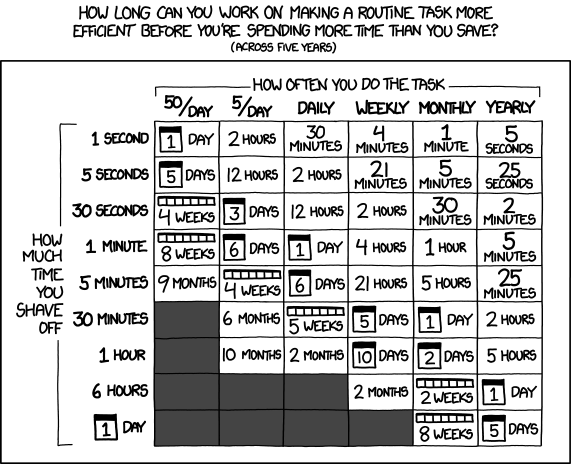
\includegraphics[height=0.9\textheight]{files/xkcd1205_is_it_worth_the_time.png}}
  \blfootnote{\url{https://xkcd.com/1205/}}
\end{frame}

\begin{frame}[plain]
  \vspace*{3ex}
  \centerline{
\includegraphics[height=0.9\textheight]{files/xkcd1319_automation.png}}
  \blfootnote{\url{https://xkcd.com/1319/}}
\end{frame}

\begin{frame}[plain]
  \centerline{\Huge Fragen?}
\end{frame}

\end{document}

